\documentclass[tikz,border=7pt]{standalone}
\usepackage[T1]{fontenc}
\usepackage{lmodern}
\usepackage{helvet}
\renewcommand{\familydefault}{\sfdefault}
\usepackage{amsmath}
\usepackage{xcolor}
\usepackage{tikz}
\usetikzlibrary{
  arrows.meta,
  positioning,
  calc,
  fit,
  shapes.geometric,
  shapes.symbols,
  backgrounds,
  decorations.pathreplacing,
  decorations.pathmorphing,
}

\definecolor{slate}{HTML}{334155}
\definecolor{teal}{HTML}{0D9488}
\definecolor{amber}{HTML}{D97706}
\definecolor{rose}{HTML}{E11D48}
\definecolor{muted}{HTML}{64748B}
\definecolor{line}{HTML}{94A3B8}
\definecolor{pagebg}{HTML}{F8FAFC}
\definecolor{card}{HTML}{FFFFFF}
\definecolor{lightteal}{HTML}{CCFBF1}
\definecolor{lightamber}{HTML}{FEF3C7}
\definecolor{lightrose}{HTML}{FFE4E6}
\definecolor{lightslate}{HTML}{E2E8F0}
\definecolor{blueink}{HTML}{2563EB}
\definecolor{bluewash}{HTML}{DBEAFE}
\definecolor{greenink}{HTML}{16A34A}
\definecolor{greenwash}{HTML}{DCFCE7}
\definecolor{pinkink}{HTML}{DB2777}
\definecolor{pinkwash}{HTML}{FCE7F3}

\tikzset{
  >=Stealth,
  font=\sffamily\scriptsize,
  every node/.append style={text=slate},
  title/.style={font=\sffamily\bfseries\small, text=slate, anchor=west},
  note/.style={font=\sffamily\tiny, text=muted, align=left},
  label/.style={font=\sffamily\tiny, text=muted},
  chip/.style={
    draw=#1,
    fill=#1!12,
    rounded corners=2pt,
    inner sep=2.5pt,
    font=\sffamily\tiny\bfseries,
    text=slate,
  },
  decision/.style={
    shape=diamond,
    aspect=2.1,
    draw=teal,
    fill=lightteal,
    inner sep=1.5pt,
    align=center,
    font=\sffamily\tiny,
    text=slate,
  },
  pics/person/.style 2 args={
    code={
      \fill[#1] (0,0.92) circle (0.18);
      \fill[#1]
        (-0.26,0.68)
        .. controls (-0.34,0.42) and (-0.30,0.18) .. (-0.22,0.02)
        -- (0.22,0.02)
        .. controls (0.30,0.18) and (0.34,0.42) .. (0.26,0.68)
        -- cycle;
      \node[font=\sffamily\tiny\bfseries, text=#1, anchor=north] at (0,-0.08) {#2};
    }
  },
  pics/disk/.style={
    code={
      \fill[lightslate] (0,-0.04) ellipse (0.28 and 0.10);
      \fill[slate] (-0.28,-0.04) rectangle (0.28,0.12);
      \fill[slate] (0,0.12) ellipse (0.28 and 0.10);
      \fill[card] (0,0.14) ellipse (0.11 and 0.04);
    }
  },
}

\begin{document}
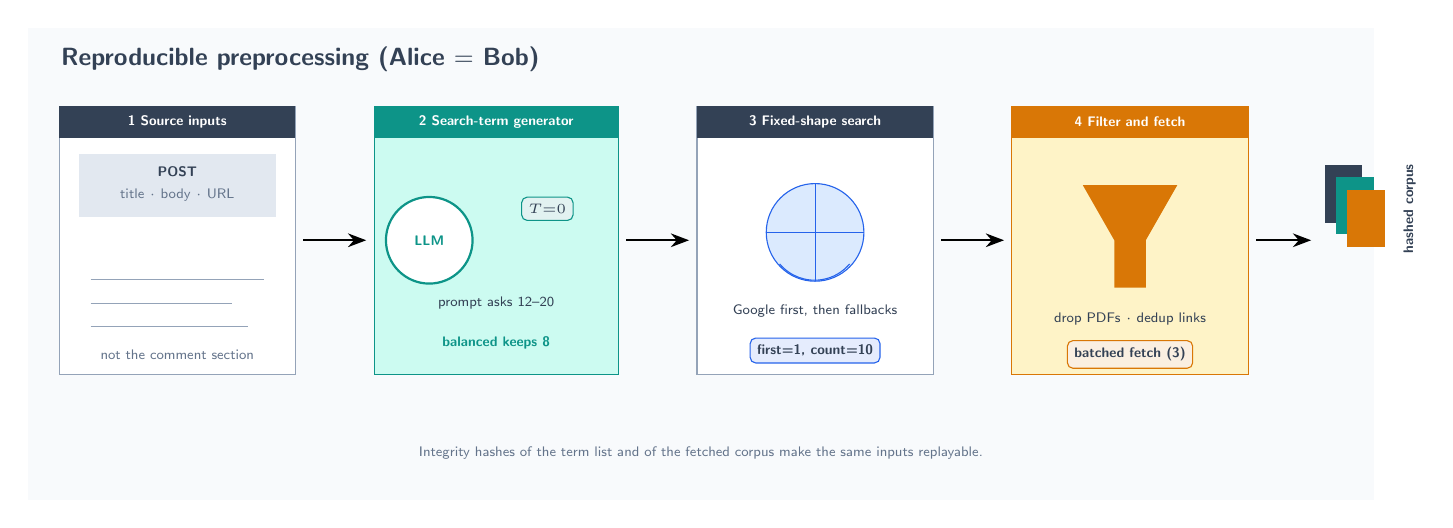
\begin{tikzpicture}[x=1cm,y=1cm]
  \fill[pagebg] (-0.25,-0.45) rectangle (16.85,5.55);
  \node[title] at (0.05,5.15) {Reproducible preprocessing (Alice $=$ Bob)};

  % 1 document
  \fill[card] (0.15,1.15) rectangle (3.15,4.55);
  \draw[line] (0.15,1.15) rectangle (3.15,4.55);
  \fill[slate] (0.15,4.15) rectangle (3.15,4.55);
  \node[font=\sffamily\tiny\bfseries, text=card] at (1.65,4.35) {1  Source inputs};
  \fill[lightslate] (0.40,3.15) rectangle (2.90,3.95);
  \node[font=\sffamily\tiny\bfseries] at (1.65,3.72) {POST};
  \node[label] at (1.65,3.42) {title $\cdot$ body $\cdot$ URL};
  \draw[line] (0.55,2.35) -- (2.75,2.35);
  \draw[line] (0.55,2.05) -- (2.35,2.05);
  \draw[line] (0.55,1.75) -- (2.55,1.75);
  \node[note, text width=2.7cm, align=center] at (1.65,1.40) {not the comment section};

  \draw[thick, ->] (3.25,2.85) -- (4.05,2.85);

  % 2 LLM
  \fill[lightteal] (4.15,1.15) rectangle (7.25,4.55);
  \draw[teal] (4.15,1.15) rectangle (7.25,4.55);
  \fill[teal] (4.15,4.15) rectangle (7.25,4.55);
  \node[font=\sffamily\tiny\bfseries, text=card] at (5.70,4.35) {2  Search-term generator};
  \fill[card] (4.85,2.85) circle (0.55);
  \draw[teal, thick] (4.85,2.85) circle (0.55);
  \node[font=\sffamily\tiny\bfseries, text=teal] at (4.85,2.85) {LLM};
  \node[chip=teal] at (6.35,3.25) {$T{=}0$};
  \node[font=\sffamily\tiny, align=center] at (5.70,2.05) {prompt asks 12--20};
  \node[font=\sffamily\tiny\bfseries, text=teal] at (5.70,1.55) {balanced keeps 8};

  \draw[thick, ->] (7.35,2.85) -- (8.15,2.85);

  % 3 search
  \fill[card] (8.25,1.15) rectangle (11.25,4.55);
  \draw[line] (8.25,1.15) rectangle (11.25,4.55);
  \fill[slate] (8.25,4.15) rectangle (11.25,4.55);
  \node[font=\sffamily\tiny\bfseries, text=card] at (9.75,4.35) {3  Fixed-shape search};
  \fill[bluewash] (9.75,2.95) circle (0.62);
  \draw[blueink] (9.75,2.95) circle (0.62);
  \draw[blueink] (9.75,2.33) -- (9.75,3.57);
  \draw[blueink] (9.13,2.95) -- (10.37,2.95);
  \draw[blueink] (9.30,2.55) arc (220:320:0.58);
  \node[font=\sffamily\tiny, align=center] at (9.75,1.95) {Google first, then fallbacks};
  \node[chip=blueink] at (9.75,1.45) {first=1, count=10};

  \draw[thick, ->] (11.35,2.85) -- (12.15,2.85);

  % 4 filter
  \fill[lightamber] (12.25,1.15) rectangle (15.25,4.55);
  \draw[amber] (12.25,1.15) rectangle (15.25,4.55);
  \fill[amber] (12.25,4.15) rectangle (15.25,4.55);
  \node[font=\sffamily\tiny\bfseries, text=card] at (13.75,4.35) {4  Filter and fetch};
  \fill[amber]
    (13.15,3.55) -- (14.35,3.55) -- (13.95,2.85) -- (13.95,2.25)
    -- (13.55,2.25) -- (13.55,2.85) -- cycle;
  \node[font=\sffamily\tiny, align=center] at (13.75,1.85) {drop PDFs $\cdot$ dedup links};
  \node[chip=amber] at (13.75,1.40) {batched fetch (3)};

  \draw[thick, ->] (15.35,2.85) -- (16.05,2.85);

  % 5 hash -- sits a bit tighter
  \begin{scope}[shift={(16.15,2.85)}]
    \fill[slate] (0.08,0.22) rectangle (0.55,0.95);
    \fill[teal] (0.22,0.08) rectangle (0.70,0.80);
    \fill[amber] (0.36,-0.08) rectangle (0.84,0.64);
    \node[font=\sffamily\tiny\bfseries, rotate=90, anchor=center] at (1.15,0.40) {hashed corpus};
  \end{scope}

  \node[note] at (8.30,0.15) {Integrity hashes of the term list and of the fetched corpus make the same inputs replayable.};
\end{tikzpicture}
\end{document}
